
\label{sec:tasks}

% \begin{figure*}[ht]
%     % \vspace{0.1in}
%     \begin{subfigure}[h]{\linewidth}
%     \includegraphics[width=0.99\textwidth, trim={0 6cm 0 1cm}, clip]{figures/tasks/basket.jpg}
%     \vspace{-2mm}
%     \caption{Lift the basket}
%     \label{fig:basket}
%     \end{subfigure}
%     \begin{subfigure}[h]{0.245\linewidth}
%     \includegraphics[width=0.99\textwidth]{figures/tasks/pull_handle.jpg}
%     \caption{Pull the Handle}
%     \label{fig:handle}
%     \end{subfigure}
%     \begin{subfigure}[h]{0.245\linewidth}
%     \includegraphics[width=0.99\textwidth]{figures/tasks/press_button.jpg}
%     \caption{Press the Button}
%     \label{fig:button}
%     \end{subfigure}
%     \begin{subfigure}[h]{0.245\linewidth}
%     \includegraphics[width=0.99\textwidth]{figures/tasks/push_door.jpg}
%     \caption{Push the Door}
%     \label{fig:interactive_reach}
%     \end{subfigure}
%     \begin{subfigure}[h]{0.245\linewidth}
%     \includegraphics[width=0.99\textwidth]{figures/tasks/valve2.jpg}
%     \caption{Twist the Valve}
%     \label{fig:valve}
%     \end{subfigure}
    
%     \begin{subfigure}{0.245\linewidth}
%     \includegraphics[width=0.99\textwidth]{figures/tasks/scrape.jpg}
%     \caption{Scrape the Object}
%     \label{fig:scrape}
%     \end{subfigure}
%     \begin{subfigure}{0.245\linewidth}
%     \includegraphics[width=0.99\textwidth]{figures/tasks/football.jpg}
%     \caption{Shoot the Ball}
%     \label{fig:football}
%     \end{subfigure}
%     \begin{subfigure}{0.245\linewidth}
%     \includegraphics[width=0.99\textwidth]{figures/tasks/washer_open1.jpg}
%     \caption{Open the Washer}
%     \label{fig:washer_open}
%     \end{subfigure}
%     \begin{subfigure}{0.245\linewidth}
%     \includegraphics[width=0.99\textwidth]{figures/tasks/washer_opened_close2.jpg}
%     \caption{Close the Washer}
%     \label{fig:washer_close}
%     \end{subfigure}
    
%     \caption{Overview of the tasks we train our robot to accomplish.}
%     \label{fig:tasks}
% \end{figure*}
\begin{figure}[]
    % \vspace{0.1in}
    % 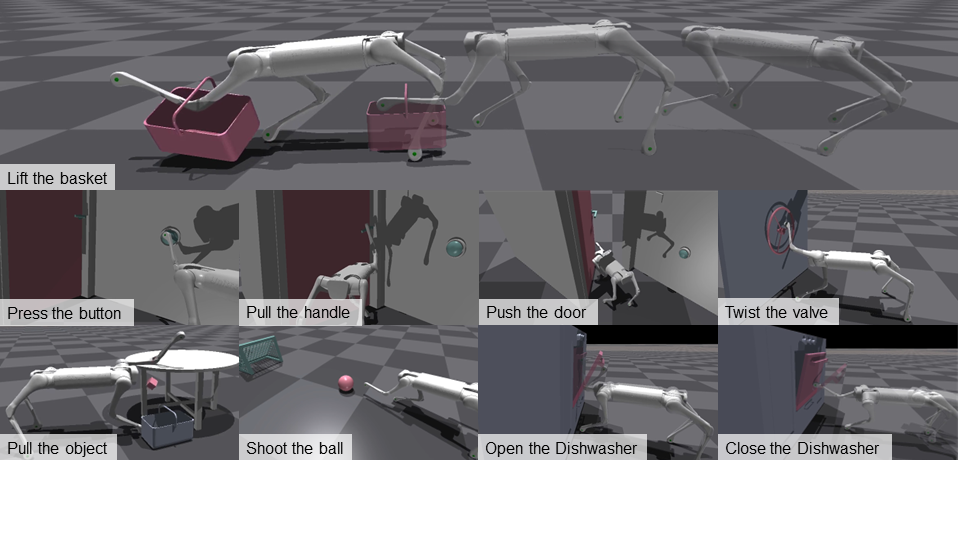
\includegraphics[width=0.99\linewidth, trim={0 5mm 0 0}, clip]{figures/tasks/all_tasks.png}
    % \centering
    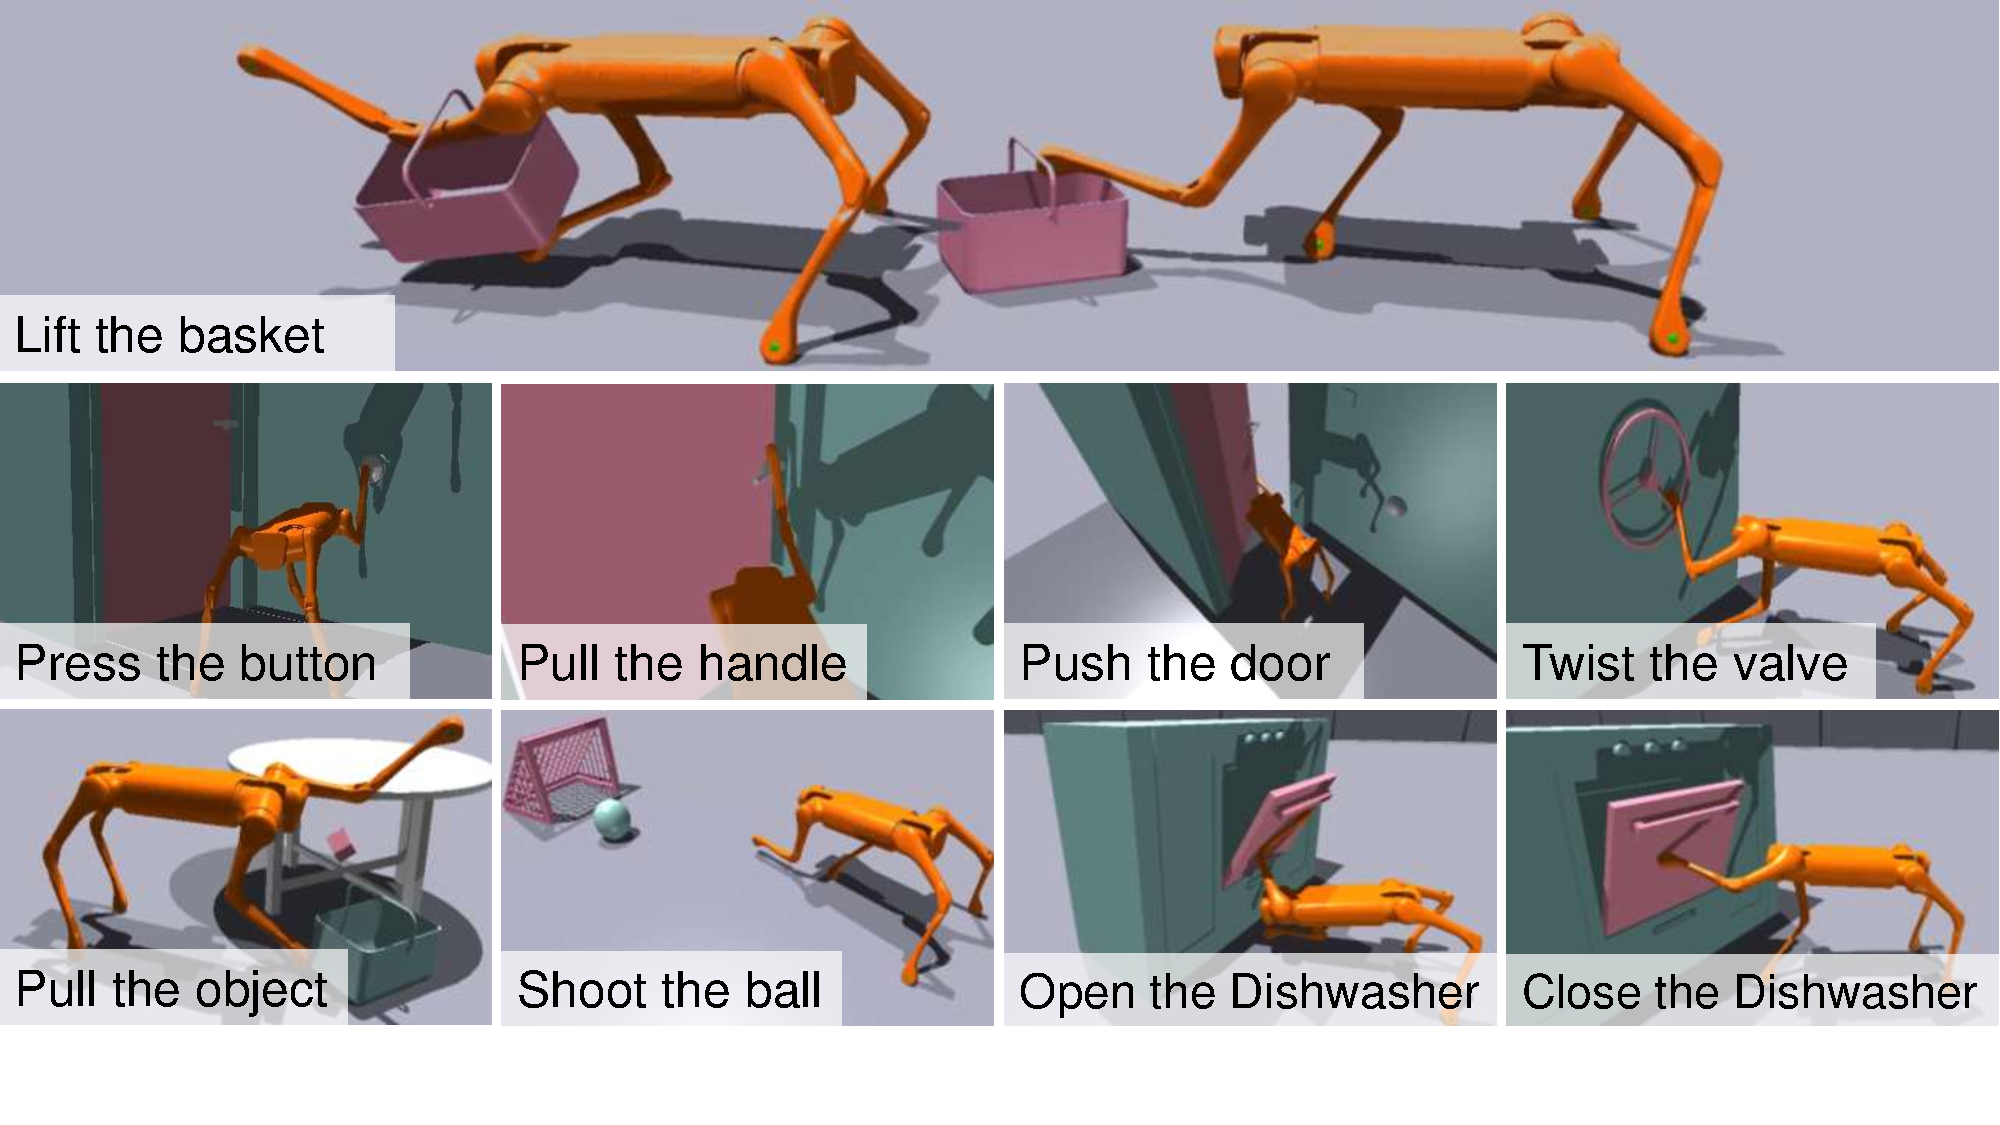
\includegraphics[width=0.99\linewidth, trim={0 17mm 0 0}, clip]{figures/tasks/all_tasks.pdf}
    % \vspace{-2mm}
    % \caption{Lift the basket}
    \label{fig:basket}
    \caption{\small Overview of the 9 loco-manipulation tasks we train our robot to accomplish. These tasks are designed to cover a large scope of the non-prehensile manipulations tasks that can be realized by the robot's leg.}
    \label{fig:tasks}
    \vspace{-.2in}
\end{figure}
There are numerous robotic manipulation benchmarks available~\cite{yu2019meta,chen2022towards,robosuite2020,RLBench}, but the majority focus on fixed-base robot manipulation. Currently, there is no suitable benchmark for assessing loco-manipulation performance. To evaluate the effectiveness of our algorithm and to provide a valuable reference for the community, we have designed a set of tasks specifically for loco-manipulation tasks, as shown in Fig.~\ref{fig:tasks}.


\subsection{Design Principles}

Based on the application scenarios and working range of legged robots, we designed a set of tasks. Solving these tasks requires the robot to perform various skills, such as pushing, tapping, pulling down, pulling out, kicking, lifting, etc. 
% These tasks encompass the daily tasks of wheeled mobile manipulators and also include tasks specifically designed for loco-manipulation. 
This allows for a comprehensive evaluation of the performance of loco-manipulators across multiple dimensions.
\subsection{Task Description}

\begin{itemize}
    \item \textbf{Press button.} The robot needs to press a hemispherical button with a diameter of 10 cm.
    \item \textbf{Pull handle.} The robot is required to pull down a door handle. Due to the height of the robot's torso and the limitations in joint angles, this task is challenging for loco-manipulation using the feet, requiring the robot to maintain high precision in manipulation at the limits of its operating space.
    \item \textbf{Push door.} The robot needs to push open a door. This assesses the ability of the robot to walk over a large distance on just three legs while manipulating the door with the foot.
    \item \textbf{Lift the Basket.} The robot needs to lift a basket with its foot and walk a distance. This evaluates the robot's precision control over the 6-DoF of its end-effector and its ability to move over a large distance.
    \item \textbf{Open dishwasher.} The robot needs to open the door of a dishwasher with its foot. This task is very easy for a robotic arm with a gripper but very difficult for a foot with point contact. 
    \item \textbf{Close the Dishwasher.} The robot needs to close the door of dishwasher with its foot.
    \item \textbf{Pull objects.} The robot is required to pull objects off a table with its foot.
    \item \textbf{Twist the Valve.} The robot has to twist a valve with a diameter of about 40 cm, where the axis is 60 cm off the ground. This tests the robot's ability to manipulate over a large range at the limits of its workspace.
    \item \textbf{Shoot ball.} The robot needs to run a distance and shoot a soccer ball into a goal with its foot.
\end{itemize}